\section{Experiments} \label{sec:experiment}
In this section, we measure the overall performance of the optimized 
OpenCL based BFS accelerator on Intel Harp-v2 
\cite{gupta2016accelerating} with a set of representative 
graphs. Then we have an end-to-end comparison to the existing OpenCL 
based BFS implementations and summarize the performance of prior BFS 
implementations on FPGAs. Finally, we analyze the proposed optimization 
methods in detail.

\subsection{Experiment Setup}
The graphs used for evaluation includes three real-world graphs and 
two synthetic graphs as listed in Table \ref{tab:graph}. The real-world 
graphs are from social network (SN) 
\cite{yang2012defining, leskovec2009community, takac2012data} while 
the synthetic graphs are generated with R-MAT model. For R-MAT graphs, 
we follow the Graph 500 benchmark parameters ($A=0.59, B=0.19, C=0.19$). 
The size of a R-MAT graph is determined by the scale 
factor $S$ and the edge factor $E$, which means the graph has $2^{S}$ 
nodes and $E\times 2^{S}$ edges.
The configurations for the two graphs R19 and R21 are $(S=19, E=32)$ and $(S=21, E=32)$ 
respectively. 
%To simplify the graph notation, the five graphs including  Youtube, Live Journal, Pokec, R-MAT$(S=19, E=32)$ and R-MAT$(S=21, E=32)$ are abbreviated to YT, LJ, PK, R19, and R21 respectively. 
In the experiments, the OpenCL compiler is based on Intel OpenCL SDK 16.1 for FPGA. 
The FPGAs used in Harp-v2 is Arria 10 GX1150\cite{gupta2016accelerating}. 
The performance metric is million traverse per second (MTEPS).
To ensure fair comparison, we tested 64 non-trivial BFS and 
averaged the the performance.  

\begin{table}
    \centering
  \caption{Graph Benchmark}
  \label{tab:graph}
  \begin{tabular}{cccc}
    \toprule
      Name & \# of vertex & \# of edge & Type \\
    \midrule
      YouTube (YT) \cite{yang2012defining} & 1,157,828 & 2,987,624 & Undirected \\
      Live Journal (LJ) \cite{leskovec2009community} & 4,847,571 & 68,993,773 & Directed \\
      Pokec (PK) \cite{takac2012data} & 1,632,804 & 30,622,564 & Directed \\
      R19 & 524,288 & 16,777,216 & Directed \\
      R21 & 2,097,152 & 67,108,864 & Directed \\
  \bottomrule
\end{tabular}
\vspace{-0.5em}
\end{table}

\subsection{Performance evaluation}
The performance of the proposed BFS accelerator i.e. OBFS 
as presented in Table \ref{tab:performance-summary} achieves 
up to 934.2 MTEPS on the R21 and 567.0 MTEPS on average 
when batch size is 16. 
Compared to the OpenCL based vertex-centric BFS 
implementation from Spector, OBFS shows 9.5X performance 
speedup, though Spector fails on the other three graphs 
due to memory access stall. 
When compared to the OpenCL based edge-centric BFS 
implementation from Chen's work \cite{chen_fpl2019}, 
OBFS achieves 5.5X performance speedup on average. 
The comparison reveals that OBFS achieves significant 
performance speedup over existing OpenCL based BFS 
implementations. 

\begin{table}
    \centering
  \caption{Performance comparison to existing OpenCL based BFS}
  \label{tab:performance-summary}
  \begin{tabular}{cccccc}
    \toprule
    Benchmark & YT & LJ & PK & R19 & R21\\
    \midrule
	OBFS & 79.4 & 475.7 & 557.8 & 787.7 & 934.2 \\
	\midrule
	Spector & 12.01 & - & - & 64 & -\\
    Speedup & 6.6X & - & - & 12.3X & - \\
	\midrule
	Work\cite{chen_fpl2019} & 25.9 & 63.9 & 81.3 & 183.5 & 157.8 \\
    Speedup & 3.1X & 7.4X & 6.8X & 4.3X & 5.9X \\
  \bottomrule
\end{tabular}
\vspace{-0.5em}
\end{table}

%The proposed design needs a coupled CPU to reorganize the RPA based on the frontier vertices.
%The process has a lot of random access and it is appropriate for CPU because 
%of the optimized cache sub system. To evaluate the approach, we further analyze the 
%execution time distribution of the BFS. According to Figure \ref{fig:runtime}, the CPU execution time 
%takes a small proportion of the whole execution time in general, while the proportion is relatively 
%higher for the social network graphs which have deeper levels and more processing on CPU 
%compared to the R-MAT graphs. 
%\begin{figure}
%	\center{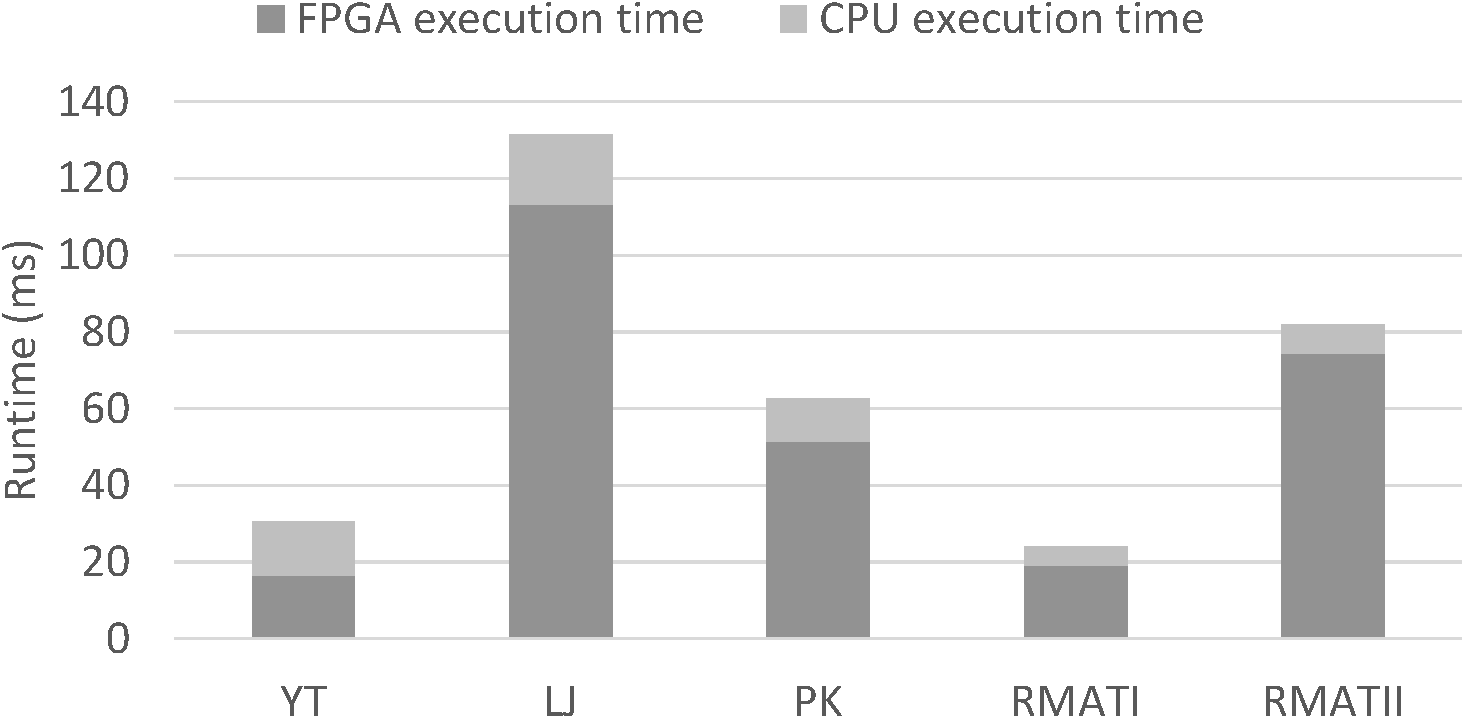
\includegraphics[width=0.85\linewidth]{runtime}}
%    \caption{Runtime distribution of the BFS accelerator on different graphs}
%\label{fig:runtime}
%\vspace{-1em}
%\end{figure}

On top of the end-to-end comparison on Harp-v2, we also compare 
OBFS to prior RTL based BFS accelerators. These BFS accelerators may 
vary on many different aspects such as graph types, memory bandwidth, 
hardware platforms, and evaluation methods. A summary of these BFS 
acceleration works is presented in Table \ref{tab:compare}.
Most of the works used either social network (SN) graphs which are the same or similar to our benchmark sets or R-MAT graphs. High-performance  
multi-FPGA platforms such as Convey HC-2 \cite{bakos2010high} have higher memory bandwidth while the single 
node machine platforms typically have relatively limited DRAM bandwidth. 
These works also differ on evaluation methods. 
Some of them obtained the performance via measurement on realistic hardware 
while others rely on simulation. 
We use 'M' and 'S' to represent the two performance evaluation methods.
 
According to the performance comparison in the Table \ref{tab:compare}, 
OBFS achieves competitive performance 
to most prior RTL designs. This demonstrates the potential of utilizing 
OpenCL for BFS with inherent irregular memory accesses. It is 
true that the performance of OBFS is not as good as that 
reported in \cite{yao2018efficient}. There may be 
mainly two reasons for this. First, current OpenCL has many 
implementation constraints which may limit the adoption of some 
optimization strategies. For instance, Current Intel OpenCL compiler 
targeting Harp-v2 does not allow on-chip buffer sharing between 
different kernels (This will be resolved in compilers supporting 
OpenCL Spec2.0, which defines global shared on-chip buffer to enable 
the feature.), so it poses constraints on BFS pipelining and 
data path parallelization. Second, OpenCL based design runs at 
lower clock frequency due to the lack of low-level circuit control 
mechanisms. For example, RTL design in \cite{yao2018efficient} runs 
at 250 MHz, but OBFS ranges from 160 MHz to 200 MHz. 
While the OpenCL tools keep evolving. it can be expected 
that the performance gap between OpenCL based designs 
and RTL designs will shrink in future. 

\begin{table}
  \footnotesize
  \caption{Performance of BFS accelerators on FPGA-DRAM platforms}
  \label{tab:compare}
    \setlength{\tabcolsep}{4pt} % Default value: 6pt
    %\renewcommand{\arraystretch}{1.5} % Default value: 1
  \begin{tabular}{cccccc}
    \toprule
	System & \shortstack[c]{Dataset \\ Type} & \shortstack[c]{Bandwidth\\ (GB/s)} & \shortstack[c]{Hardware\\ Platform} & \shortstack[c]{Design\\ Method} & \shortstack[c]{MTEPS\\ /FPGA}\\
    \midrule
	Work\cite{wang2010message} & SN & 0.1 & Virtex-5 & S\&RTL & 160-790 \\
	Work\cite{betkaoui2012reconfigurable} & fMRI & 80 & HC-2 & M\&RTL & 62.5-650 \\
	CyGraph\cite{attia2014cygraph} & R-MAT & 80 & HC-2 & M\&RTL & 420-550 \\
	Work\cite{umuroglu2015hybrid} & R-MAT & 3.2 & Zedboard & M\&RTL & 90-255 \\
	FPGP\cite{dai2016fpgp} & SN & 12.8 & VC707 & M\&RTL & 122 \\
	ForeGraph\cite{Dai2017foregraph} & SN &19.2 & VCU110 & S\&RTL & 364-1069 \\
	%2017 & Jialiang's work\cite{zhang2017boosting} & AC-510 & 130-166 & M/S\&RTL \\
	Work\cite{zhou2017accelerating} & R-MAT & 12.8 & Harp-v1 & M\&RTL & 330-670 \\
	%2018 & Jialiang's work \cite{zhang2018degree} & AC-510 & 400-1526 & M/S\&RTL \\
	%2018 & Soroosh's work \cite{khoram2018accelerating} & AC-510 & 100-650 & M\&RTL\\
	Work\cite{yao2018efficient} & SN & 19.2 & Ultrascale+ & S\&RTL & 1500-3500 \\
	\midrule
	%Spector \cite{gautier2016spector} & R-MAT & 16 & Harp-v2 & M\&OCL & 64 \\
	%Spector \cite{gautier2016spector} & SN & 16 & Harp-v2 & M\&OCL & 12 \\
	%Work\cite{chen_fpl2019} & R-MAT & 16 & Harp-v2 & M\&OCL & 171 \\
	%Work\cite{chen_fpl2019} & SN & 16 & Harp-v2 & M\&OCL & 57 \\
	%2018 & GraFBoot\cite{jun2018grafboost} & VC707+Flash & 57-75 & M\&RTL\\
	%2019 & baseline (R-MAT Graph) & Harp-v2 & 58.3 & M\&OCL \\
	%2019 & baseline (Social Network) & Harp-v2 & 44.2 & M\&OCL \\
	OBFS & R-MAT & 16 & Harp-v2 & M\&OCL &  861 \\
	OBFS & SN & 16 & Harp-v2 & M\&OCL & 371 \\
  \bottomrule
\end{tabular}
\vspace{-1em}
\end{table}

\subsection{OpenCL optimization analysis}
In this work, we mainly apply three different approaches including 
memory coalescing, on-chip bitmap buffering and level update shifting 
to optimize the OpenCL based BFS accelerator. While the memory coalescing is 
a combination of data alignment, graph reordering and batching as well as 
spatial data path parallelization and they are dependent, 
we have them evaluated together. By increasingly deploying the optimization 
approaches to the base BFS accelerator (baseline) which is the five-stage pipelined BFS 
accelerator discussed in Section~\ref{sec:overview}, the performance improvement of each 
optimization can be obtained as presented in Figure \ref{fig:opt-analysis}. 
Note that the accelerators with different optimization approaches have 8Mb 
bitmap implemented. Batch size is set to be 16. It can be found that the 
graph memory coalescing contributes most to the overall performance improvement. 
%Bitmap buffering and level update shifting exhibit less significant 
%performance improvement. 

 \begin{figure}
	\center{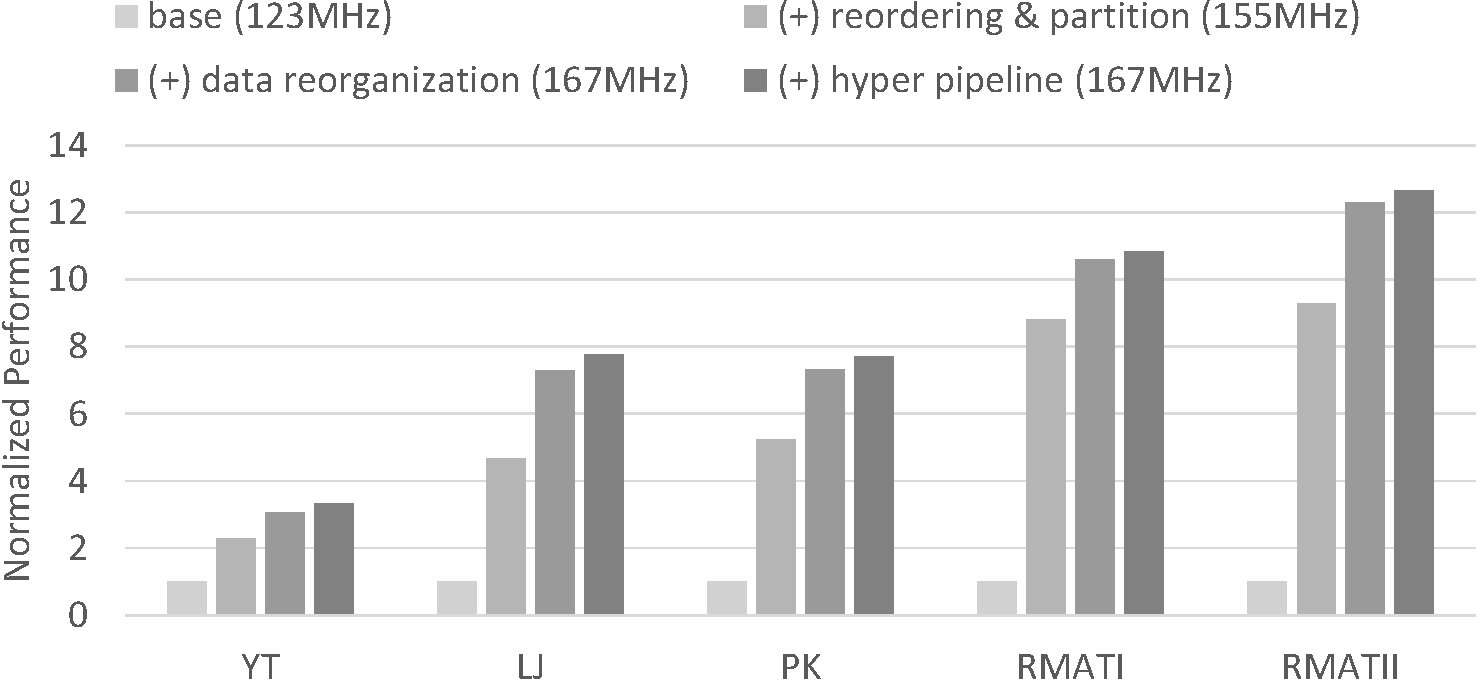
\includegraphics[width=0.75\linewidth]{opt-analysis}}
	\caption{Performance improvement of BFS with different optimizations}
\label{fig:opt-analysis}
\vspace{-1em}
\end{figure}

%When different optimization approaches are applied to the OpenCL based 
%BFS accelerators, the clock frequency of the implementations are different, 
%which also affects the BFS performance. The clock frequency of the implementations 
%with different optimization approaches is given in Table \ref{tab:opt-freq}. 
%Since bitmap buffer size also affects the clock frequency of the implementations, 
%we present two typical setups i.e. 4Mb and 8Mb bitmap buffers in the table. 
%According to the experiments, the achieved clock frequency increases when 
%on-chip bitmap buffering and level update shifting are adopted, which also 
%contribute to the performance.

%\begin{table}
%	\vspace{-1em}
%  \caption{Clokc frequency of BFS implementations with different high-level optimizations}
%  \label{tab:opt-freq}
%    \setlength{\tabcolsep}{4pt} % Default value: 6pt
%    %\renewcommand{\arraystretch}{1.5} % Default value: 1
%	\centering
%  \begin{tabular}{ccccc}
%    \toprule
%	bitmap & base & \shortstack{(+) memory\& \\ coalescing} & \shortstack{(+)bitmap \\ buffering} & \shortstack{(+)level \\ update shifting} \\
%	\midrule
%	4Mb & 123 MHz & 155 MHz & \textbf{xxx} MHz & 202 MHz\\
%	8Mb & 110 MHz & 142 MHz & \textbf{xxx} MHz & 165 MHz\\
%  \bottomrule
%\end{tabular}
%\vspace{-1em}
%\end{table}

Since memory coalescing contributes most to the performance and we further analyze 
its main design parameter i.e. the batch size, which determines the amount of 
padding to the graph and the number of parallel processing units.
Given different batch sizes, BFS performance is shown in Figure \ref{fig:batch-perf}.
The performance increases with the batch size first, and it starts to drop after reaching 
the optimal batch size. The optimal batch size turns out to be 16 for the five graphs. 
Larger batch size indicates more parallel processing units and larger aligned 
memory requests, which improves the memory bandwidth utilization and promises 
better performance. 

\begin{figure}
	\center{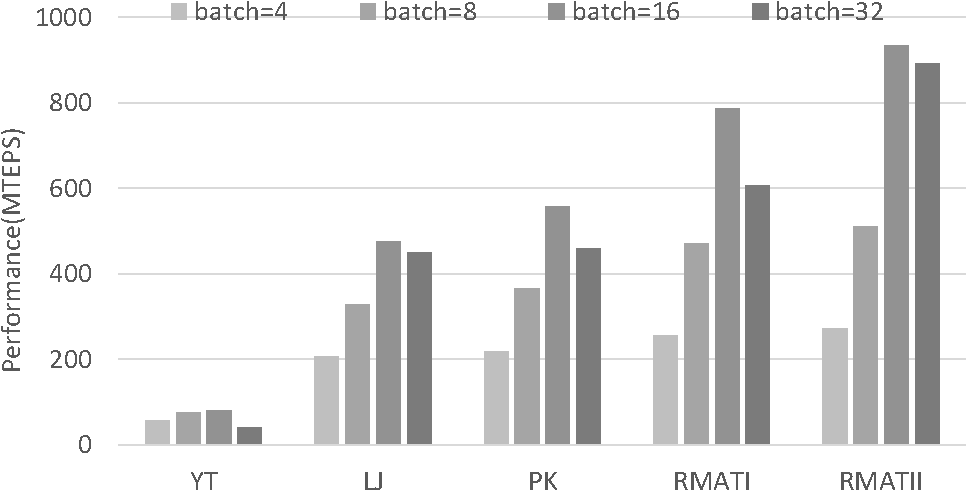
\includegraphics[width=0.72\linewidth]{batch-perf}}
    \caption{Performance of OBFS with different batch sizes}
\label{fig:batch-perf}
\vspace{-1em}
\end{figure}

The disadvantage of having a larger batch size is to incur more padding to 
the graphs, which may waste the memory bandwidth. 
The relative CSR data size after batching is illustrated in Figure \ref{fig:batch-overhead}. 
It can be found that the batched CSR data size of R-MAT graphs with larger average 
degree is much smaller than that of the social network graphs with lower average degree.
When batch is 16, the normalized CSR data size for R-MAT graphs is roughly 2X, the normalized data size 
for LJ and PK is around 4X larger and the normalized data size for YT with the lowest average degree 
is over 6X. Basically, graphs with lower degree include large portion of low-degree 
vertices which have insufficient neighbors to construct even an aligned batch. As a result, 
a lot of padding i.e. '-1' are inserted and the data size goes up dramatically. 
They induce additional memory accesses and degrade BFS performance eventually.
The trend of the BFS performance with increasing batch size essentially 
shows the trade-off between the above advantages and disadvantages.

\begin{figure}
	\center{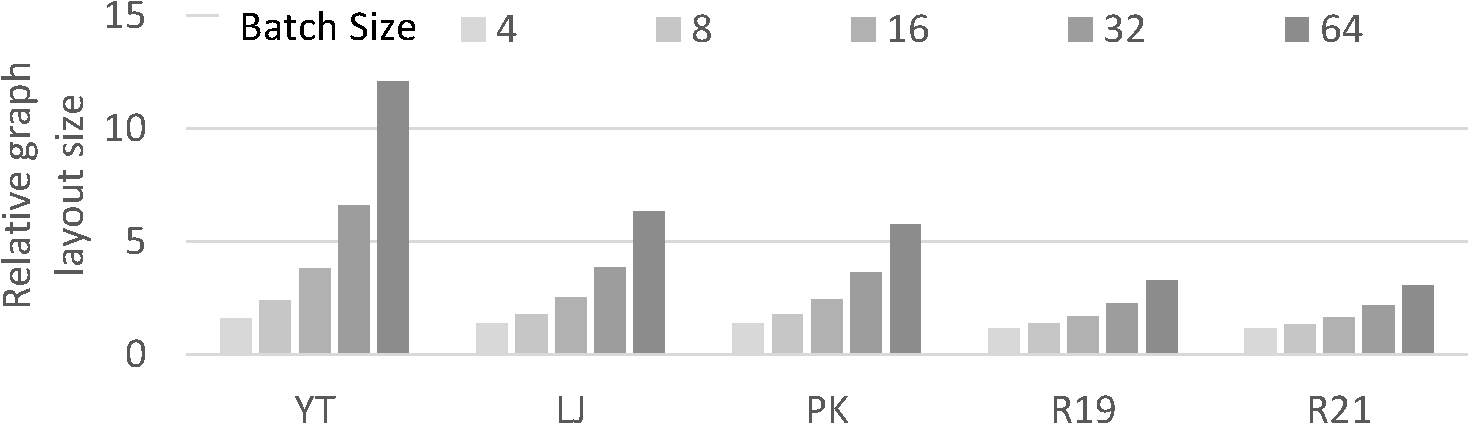
\includegraphics[width=0.72\linewidth]{batch-overhead}}
    \caption{Relative CSR data size with different batch sizes}
\label{fig:batch-overhead}
\vspace{-1em}
\end{figure}

%The advantages of the batch are multi-folded.
%In particular, batch mainly has the memory 
%access coalesced and improves the memory bandwidth utilization, 
%In combination with the bitmap, the irregular memory access 
%reduces by more than 90\% compared to the base design.
%Batched memory access has much lower average latency. 
%To trade-off the batch overhead and the performance benefit, 
%larger batch size is recommended for graphs with higher average degree 
%and smaller batch size is better for graphs with lower degree 
%such as YT.  


%For sequential memory access and random access, 
%we performed independent experiments on Harp-v2 
%to evaluate the benefits. We measured the transfer time 
%of 64MB data in different batch size and calculated the 
%corresponding bandwidth. The bandwidth is normalized to 
%the transfer with 32-bit data width. The relative bandwidth result is presented in 
%Figure \ref{fig:mem-bandwidth}. Note that dependent random access pattern 
%refers to the random accesses that can only proceed one after another.
%This happens in the OpenCL based BFS. As low-degree frontier 
%vertices in each data path traverse sequentially because the compiler 
%has no clue if there is data dependency between different frontier 
%neighbors. 
%
%\begin{figure}
%	\center{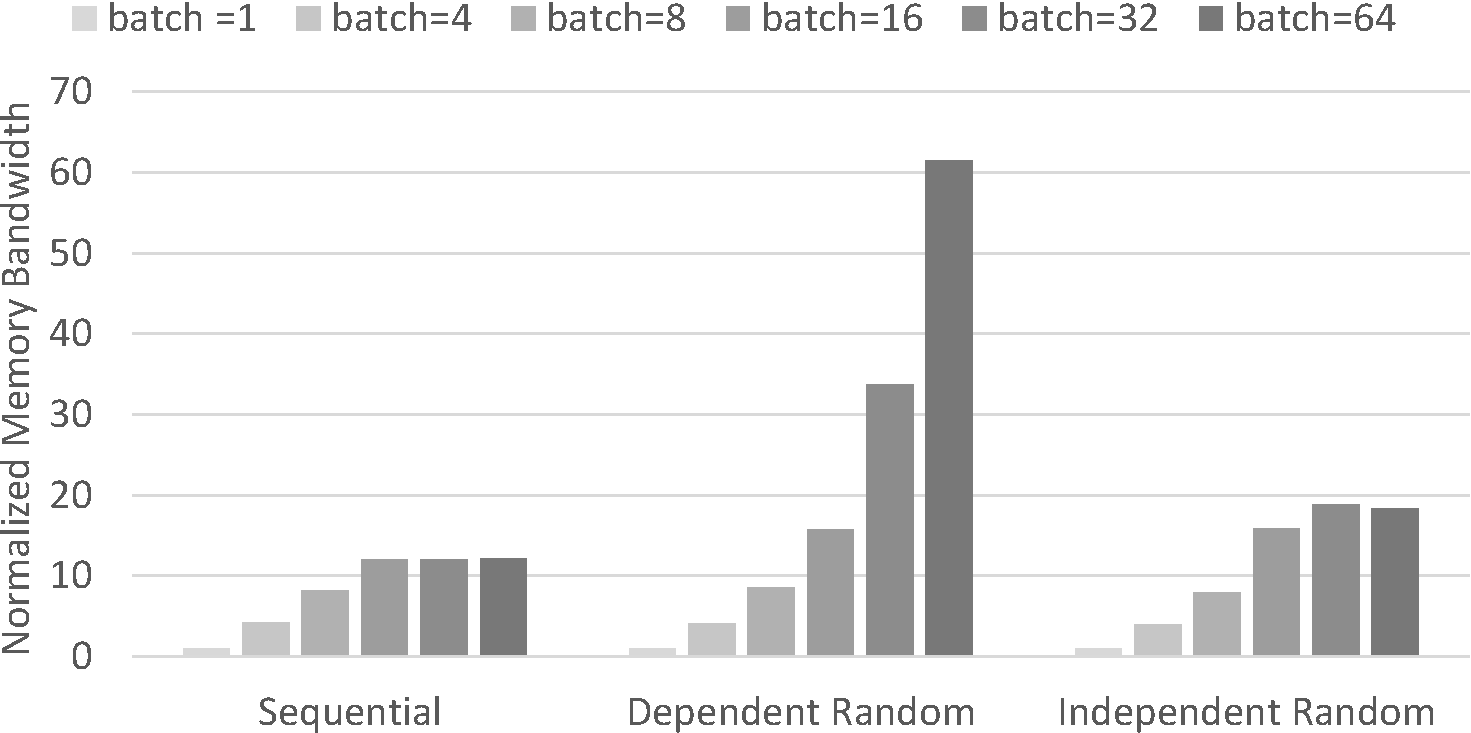
\includegraphics[width=0.85\linewidth]{mem-bandwidth}}
%    \caption{Batch size influence on memory bandwidth}
%\label{fig:mem-bandwidth}
%\vspace{-1em}
%\end{figure}


%It is clear that the bandwidth utilization of batched random memory access
%improvement is significantly higher than that of the sequential memory access. 
%Particularly, dependent random memory access keeps continuous memory 
%bandwidth utilization improvement when the batch size goes up to 64,
%While the independent random memory access gets saturated when 
%the batch size reaches to 32. It indicates that the OpenCL tools 
%can actually explore memory level parallelism of random memory access.
%For sequential memory access, the bandwidth utilization saturates 
%when the batch size is 16 and the data width equals to the 
%internal 512 bit. In general, the experiment exhibits the potential 
%memory bandwidth utilization improvement of BFS using the proposed 
%reordering and batching.

\subsection{Hardware implementation}
The FPGA resource consumption and the implementation frequency of 
OBFS are listed in Table \ref{tab:resource}. Bitmap size and batch 
size are the main OBFS design parameters that affect the hardware 
implementation. Various combinations of the two parameters are 
presented.

As shown in Table \ref{tab:resource}, built-in firmware in Harp-v2 consumes 
a large portion of the FPGA resources. In contrast, the logic cell 
consumption of OBFS is small and increases with batch size 
which means more parallel processing units. As for the on-chip 
RAM blocks, BFS accelerator with 16Mb bitmap buffer actually takes 
around 47\% of the total RAM blocks while 32 Mb bitmap fails to be fitted 
due to the built-in firmware overhead. Larger batch size which 
indicates smaller bitmap partitions is more friendly to 
the FPGA placement and beneficial to the FPGA 
implementation frequency. While bitmap size has 
negative influence on the hardware implementation frequency, 
we tend to choose the BFS accelerators with just enough 
bitmap buffer for a specific graph to obtain higher 
implementation frequency and performance.

\begin{table}
  \footnotesize
  \caption{FPGA resource consumption of OBFS with different configurations}
  \label{tab:resource}
  %\setlength{\tabcolsep}{4pt} % Default value: 6pt
  %\renewcommand{\arraystretch}{1.5} % Default value: 1
    \centering
  \begin{tabular}{cccc}
    \toprule
	\shortstack{Config. \\ (batch, bitmap)} & \shortstack{Logic \\ Resource} & \shortstack{RAM \\ blocks} & \shortstack{Frequency \\ (MHz)} \\
	\midrule
	  bare platform   & 24\% & 8\%  & -   \\
	  \midrule
	  (4, 4Mb)   & 29\% & 26\% & 158 \\
	  (8, 4Mb)   & 32\% & 27\% & 172 \\
	  (16, 4Mb)  & 37\% & 28\% & 201 \\
	  (32, 4Mb)  & 49\% & 29\% & 208 \\
	  \midrule
	  (4, 8Mb)  & 28\% & 36\% & 144 \\
	  (8, 8Mb)  & 31\% & 36\% & 153 \\
	  (16, 8Mb) & 37\% & 38\% & 165 \\
	  (32, 8Mb) & 48\% & 40\% & 177 \\
	  \midrule
	  (4, 16Mb)  & 28\% & 55\% & 132 \\
	  (8, 16Mb)  & 31\% & 55\% & 128 \\
	  (16, 16Mb) & 37\% & 57\% & 148 \\
	  (32, 16Mb) & 48\% & 59\% & 149 \\
	  \midrule
      Spector    & 39\% & 36\% & 190 \\
  \bottomrule
\end{tabular}
\vspace{-1em}
\end{table}

\subsection{Design portability}
OBFS inherits the portability from OpenCL language and porting OBFS 
to a different FPGA platform is much easier compared to 
porting RTL designs. The run-time environment and drivers provided 
by the vendors further improve the portability. Still, the ease of porting OBFS
varies depending on the target FPGA platforms and the user's experiences. 
As a sanity check, we perform a study to port the OpenCL code to other FPGA platforms.
As an experienced user with basic knowledge of both Intel OpenCL and 
Xilinx HLS tools, it took us no time to port OBFS to Harp-v2 with newer 
FPGA devices. To port OBFS to Intel FPGA platforms with independent 
DRAM such as Intel DE-5, we need to replace the shared 
memory communication approach with explicit copy. It took us around half an hour
to complete. To port OBFS to Xilinx FPGA platform such as KCU1500, we need to 
adapt to the different Vendor specific APIs, data flow coding style, optimization 
pragma and vendor specific constraints such as kernel number limitation, it took us 
around 3 hours to complete. This preliminary case study demonstrates the portability 
of our design. It is our future work to further investigate this portability with more users and more primitives.

